\documentclass{article}
\usepackage[left=2.3cm, right=2.3cm, top=1.7cm, bottom=1.7cm]{geometry}



\usepackage{tikz}
\usepackage{mhchem}
\usepackage{color}


\usepackage{Sweave}
\begin{document}
\input{practice_test-SOLUTIONS-concordance}

{\Large \textbf{Name:}} \hspace{3cm} \vspace{1cm}


\begin{center}
{\Huge Year 11 Chemistry}
\end{center}

\begin{center}
{\huge Acids and Bases Practice Test}
\end{center}

\begin{center}
{\huge {\color{red} Solutions}}
\end{center}


{\Large

\vspace{0.2cm}
\hspace{1cm}
\textbf{Question 1} 
\vspace{0.2cm}

Carbonic Acid, \ce{H_2CO_3}, is a diprotic acid.
\vspace{0.2cm}

\textbf{(a)} Write two equations to show the stages of its ionisation.

{\color{red}
\begin{center}
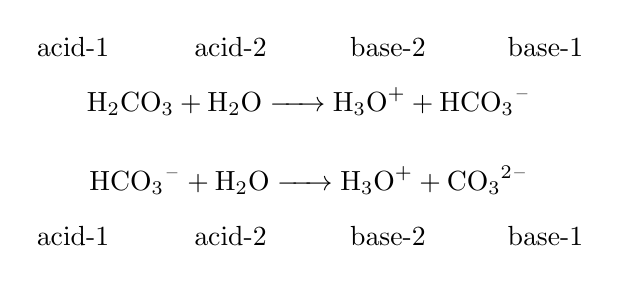
\begin{tikzpicture}
  \draw (0,1) node {\ce{H_2CO_3 + H_2O -> H_3O^+ + HCO_3^-}};
  \draw (0,0) node {\ce{HCO_3^- + H_2O -> H_3O^+ + CO_3^2-}};
  
  \draw (-3,1.7) node {acid-1};
  \draw (3,1.7) node {base-1};
  \draw (-1,1.7) node {acid-2};
  \draw (1,1.7) node {base-2};

  \draw (-3,-0.7) node {acid-1};
  \draw (3,-0.7) node {base-1};
  \draw (-1,-0.7) node {acid-2};
  \draw (1,-0.7) node {base-2};
\end{tikzpicture}
\end{center}
}

\textbf{(b)} Label the conjugate acid-base pairs in the equations above.
\vspace{0.2cm}

\textbf{(c)} State one substance from the equations above that is amphiprotic.
\vspace{0.2cm}

{\color{red}
Hydrogen Carbonate: \ce{HCO_3^-} acts as a base in the top equation, and as an acid in the bottom equation. It is amphiprotic because it can act as either an acid or a base.
}
\vspace{0.2cm}

\textbf{(d)} Explain how \ce{H_2CO_3} is acting as an acid in one of the equations above.
\vspace{0.2cm}

{\color{red}
In the top equation carbonic acid (\ce{H_2CO_3}) donates a proton to the water (\ce{H_2O}), and is thereby acting as an acid (a proton donor).
}

\vspace{0.2cm}
\hspace{1cm}
\textbf{Question 2} 
\vspace{0.2cm}

Potasium oxide, \ce{K_2O}, is a base. Write its hydrolysis (reaction with water) equation and use this equation to explain why it is a base.
\vspace{0.2cm}

{\color{red}
\begin{center}
  \ce{K_2O + H_2O -> 2OH^- + 2K^+}
\end{center}

The potassium oxide (\ce{K_2O}), formed out of two potassium (\ce{K^+}) and one oxide (\ce{O^2-}) ions absorbs a proton (\ce{H^+}) to form hydroxide (\ce{OH^-}). This could also be written as 

\begin{center}
  \ce{K_2O + H_2O -> KOH + OH^- + K^+}
\end{center}

The only difference between the two are if the potassium hydroxide is written in ionised form (i.e. \ce{KOH -> K^+ + OH^-}).
}


\pagebreak
\vspace{0.2cm}
\hspace{1cm}
\textbf{Question 3} 
\vspace{0.2cm}

\textbf{(a)} In the laboratory, an unknown white powder is suspected to be either a metal or metal carbonate of some kind. When a small amount is added to hydrochloric acid (\ce{HCl}), bubbles of gas are produced rapidly. Describe clearly the procedures you could use to identify the gas and hence rule out that it is either a metal or a metal carbonate.
\vspace{0.2cm}

{\color{red}
If the powder was a metal, it would likely react with the hydrochloric acid (\ce{HCl}) to form hydrogen gas (\ce{H_2}). If it was a carbonate it would likely react to form carbon dioxide (\ce{CO_2}).

I would capture some of the gas, and expose it to an open flame. If there is a 'pop', it indicates the gas is flammable and might be hydrogen (\ce{H_2}). If it does not 'pop', then it is not hydrogen gas and hence we can probably rule out that the power is a metal.

In that case, I would bubble the gas slowly through some limewater, i.e. a solution of calcium carbonate (\ce{CaCO_3}). If the solution goes cloudy, this indicates the gas could be carbon dioxide (\ce{CO_2}).  If the solution does not go cloudy, the has is likely not carbon dioxide (\ce{CO_2}), and so we can probably rule out the powder being a carbonate.
}
\vspace{0.2cm}

\textbf{(b)} Write the equation for the reaction between hydrochloric acid (\ce{HCl}) and magnesium metal (\ce{Mg}).

{\color{red}
\begin{center}
  \ce{2HCl + Mg -> H_2 + MgCl_2}
\end{center}
}


\textbf{(c)} Write the equation for the reaction between hydrochloric acid (\ce{HCl}) and magnesium carbonate (\ce{MgCO_3}).

{\color{red}
\begin{center}
  \ce{2HCl + MgCO_3 -> CO_2 + H_2O + MgCl_2}
\end{center}
}

\pagebreak
\vspace{0.2cm}
\hspace{1cm}
\textbf{Question 4} 
\vspace{0.2cm}

Write balanced equations for these reactions:
\vspace{0.2cm}

\textbf{(a)} Calcium Hydroxide (\ce{Ca(OH)_2}) and sulfuric acid (\ce{H_2SO_4}).

{\color{red}
\begin{center}
  \ce{Ca(OH)_2 + H_2SO_4 -> 2H_2O + CaSO_4}
\end{center}
}

\textbf{(b)} Ammonia (\ce{NH_3}) and phosphoric acid (\ce{H_3PO_4}).

{\color{red}
\begin{center}
  \ce{3NH_3 + H_3PO_4 -> (NH_4)_3PO_4}
\end{center}
}

\textbf{(c)} Alumina or aluminum oxide (\ce{Al_2O_3}) hydrochloric acid (\ce{HCl}).

{\color{red}
\begin{center}
  \ce{Al_2O_3 + 6HCl -> 3H_2O + 2AlCl_3}
\end{center}
}

\pagebreak
\vspace{0.2cm}
\hspace{1cm}
\textbf{Question 5} 
\vspace{0.2cm}

Describe clearly, with the use of a diagram to aid if helpful, why you can have dilute carbonic acid (\ce{H_2CO_3}) solution and concentrated carbonic acid solution, even though carbonic acid is said to be a "weak" acid.
\vspace{0.2cm}

{\color{red}
Because the "weakness" or "strength" of an acid only has to do with how likely it is to ionise in a solution of water --- i.e. how much of it will exist as ions in solution. Concentration on the other hand, has to do ith how much of the acid there is in relation to the amount of water. So you can have either a concentrated or dilute solution of a "weak" acid like carbonic acid (\ce{H_2CO_3}), simply by adjusting the ratio of acid to water, as the degree to which the acid ionises in solution --- i.e. the "weakness" of the acid --- will have no impact on it's concentration.
}

\pagebreak
\vspace{0.2cm}
\hspace{1cm}
\textbf{Question 6} 
\vspace{0.2cm}

Calculate the pH of the following:
\vspace{0.2cm}

\textbf{(a)} A solution in which the concentration of \ce{H_3O^+} is $10^{-4}$M.

{\color{red}
\begin{align*}
  pH  &= -\text{log}([\text{\ce{H_3O^+}}]) \\
      &= -\text{log}(10^{-4}) \\
      &= -(-4) \\
      &= 4
\end{align*}
}

\textbf{(b)} A solution in which the concentration of \ce{H_3O^+} is $3.2 \times 10^{-5}$M.

{\color{red}
\begin{align*}
  pH  &= -\text{log}([\text{\ce{H_3O^+}}]) \\
      &= -\text{log}(3.2 \times 10^{-5}) \\
      &= -(-4.49485) \\
      &\approx 4.5
\end{align*}
}

\textbf{(c)} A solution of $1.7 \times 10^{-3}$M sulphuric acid (\ce{H_2SO_4}).

{\color{red}
\begin{center}
  \ce{H_2SO_4 + 2H_2O -> 2H_3O^+ + SO_4^2-}
\end{center}

so

\begin{align*}
  \ce{H_2SO_4}&:H_3O^+ \\
  1&:2, \text{ so} \\
  [H_3O^+]&= 2 \times [H_2SO_4] \\
          &= 2 \times 1.7 \times 10^-3 \\
          &= 3.4 \times 10^-3, \text{ , and so} \\
  pH  &= -log([\ce{H_3O^+}]) \\
      &= -log(3.4 \times 10^-3) \\
      &= -(-2.46852) \\
      &\sim 2.5
\end{align*}
}

\pagebreak
\textbf{(d)} What assumptions have you made in your calculation in part (c) above? Are these assumptions reasonable in this case?
\vspace{0.2cm}

{\color{red}
We are assuming that 100\% of the Sulfuric acid (\ce{H_2SO_4}) is ionised in solution, i.e. it all exists as hydronium (\ce{H_3O^+}) and sulfate (\ce{SO_4^2-}) ions and none of it exists in solution as the acid form (\ce{H_2SO_4}). This is to say, we are assuming that sulfuric acid is a very \textbf{strong} acid.

}

}
\end{document}
